%\part*{Lezione 21/04/2021}
\paragraph{Nel dettaglio}
Discutiamo adesso i singoli \textit{step} del metodo.
\begin{enumerate}[\textbf{Step} I.]
	\item Scegliamo un opportuno \vir{cavallo} (come studiato precedentemente).
	\item Settiamo l'energia del fascio e le condizioni iniziali in modo tale che:
	\begin{enumerate}[(a)]
		\item la velocità sia tale da superare la barriera coulombiana, ma rimanga limitata da quella di Fermi.
		\item la cinematica rimanga quasi-\textit{free}.
	\end{enumerate}
	\noindent Per quanto riguarda quest'ultimo punto prendiamo a esempio:
	$$\underbrace{d}_{p-n} + \ce{^{18}O} \to \ce{^{15}N} + \alpha + n$$
	Questo è il processo che vorremmo, tuttavia se il neutrone non è spettatore potremmo avere gli stessi prodotti, ma con una reazione differente, come riportato in Figura \ref{0421_sch}. 
	\begin{figure}[h]
		\centering
		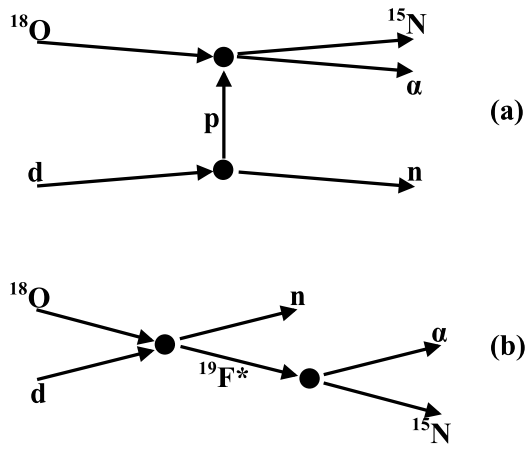
\includegraphics[scale=0.5]{Immagini/0421_sch-cut1.png}
		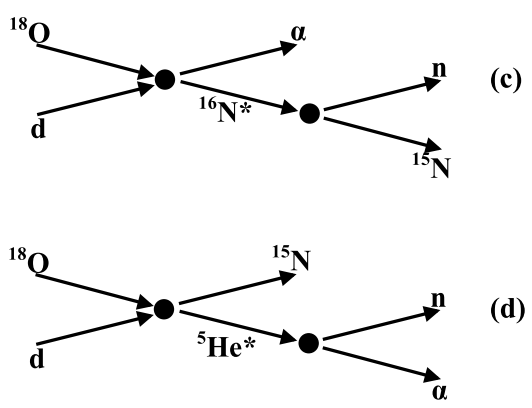
\includegraphics[scale=0.5]{Immagini/0421_sch-cut2.png}
		\caption{Possibili processi di reazione di $d+\ce{^{18}O}$. Solo nel caso (a) il neutrone è spettatore.}
		\label{0421_sch}
	\end{figure}
	\noindent Questi processi \vir{sporcano} la misura, quindi è necessario trovare un modo per riconoscerli; notiamo che ognuno passa per un \textit{compound nucleus}\index{compound nucleus@\textit{compound nucleus}} ($\ce{^{19}F}^*, \ce{^{16}N}^*,\ce{^5He}^*$) per cui sono facilmente individuabili attraverso gli \textit{energy correlation spectra}\index{energy correlation spectra@\textit{energy correlation spectra}} da un picco di risonanza che non compare nella reazione cercata. Ne riportiamo un esempio in Figura \ref{0421_spec-W} (a sinistra). Individuate le energie di risonanza si mettono dei tagli così si \vir{ripulisce} il fascio.
	\begin{figure}[h]
		\centering
		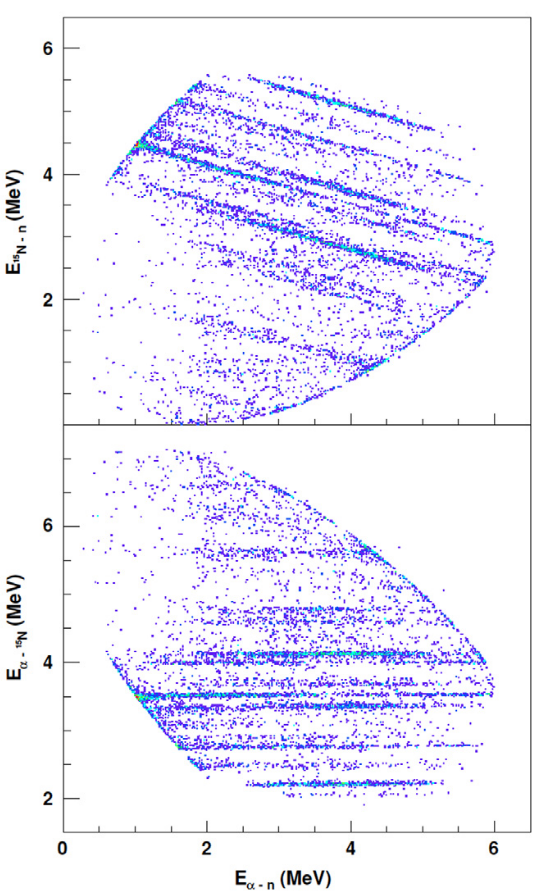
\includegraphics[scale=0.5]{Immagini/0421_eng.png}
		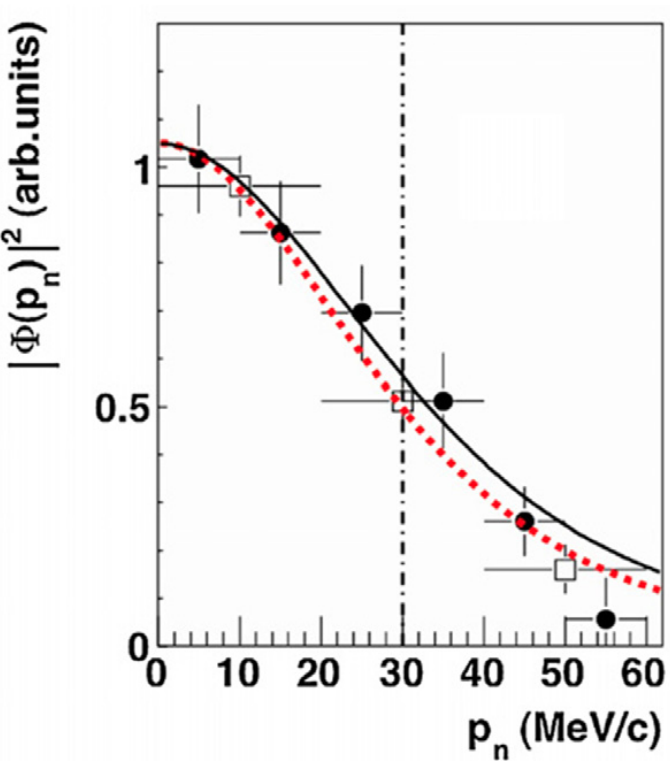
\includegraphics[scale=0.5]{Immagini/0421_pn.png}
		\caption{A sinistra \textit{energy correlation spectra}: energia relativa tra $\alpha$ e $\ce{^{15}N}$ contro quella tra $\alpha$ e $n$. Nel riquadro in basso i fasci orizzontali corrispondono agli stati eccitati del $\ce{^{19}F}^*$. A destra distribuzione dei momenti, con $\Phi\equiv W$: i pallini sono i dati sperimentali, in rosso tratteggiata è la teoria in PWBA, mentre in nero continua è un fit con parametri liberi.}
		\label{0421_spec-W}
	\end{figure}
	\item Dobbiamo conoscere $|W(\vec{P}_{bx})|^2$ e per far questo ci sono 2 strade:
	\begin{itemize}
		\item viene calcolato (caso di nuclei leggeri);
		\item oppure si sviluppa prima una teoria di scattering e poi si misura.
	\end{itemize}
	Nel secondo caso si può ottenere la misura facendo uno scattering in un certo range di energie. Prendiamo come esempio la reazione:
	$$ \underbrace{d}_{p-n} + \ce{^{11}B} \to \ce{^{8}Be} +\alpha +n $$ 
	I risultati sono riportati in Figura \ref{0421_spec-W} (a destra).
	\vspace{-1cm}
	\begin{figure}[!h]
		\centering
		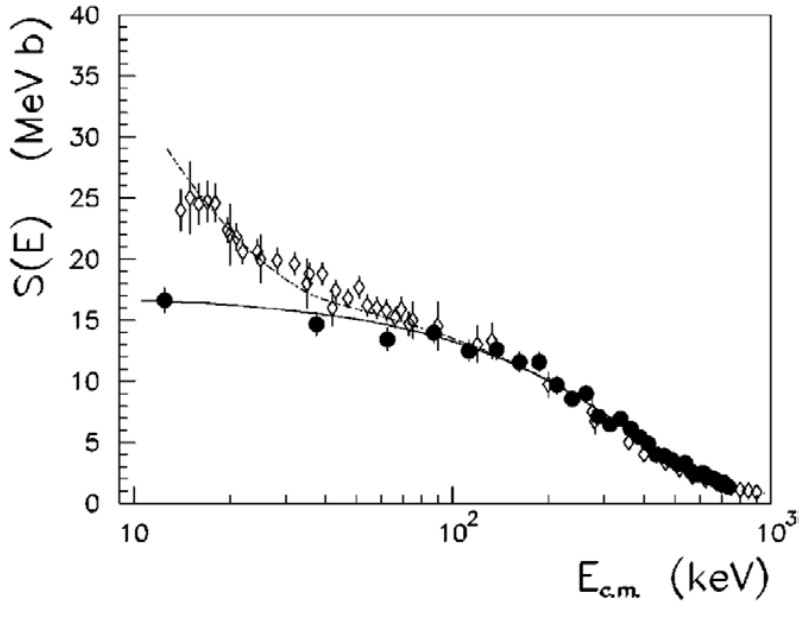
\includegraphics[scale=0.5]{Immagini/0421_Se.png}
		\caption{Fattore astrofisico per $\ce{^6Li} + \ce{^6Li}$: i puntini neri sono ottenuti con THM, i punti vuoti sono i dati sperimentali, la linea continua nera è un fit. Il \textit{gap} a basse energie è dovuto all'elettroscreening\index{elettroscreening}, non considerato dalla teoria del THM.}
		\label{0421_Se}
	\end{figure}	
\end{enumerate}
\paragraph{Fattore astrofisico} Effettivamente ciò che si misura è $\frac{d^3\sigma}{dE_c d\Omega_cd\Omega_{C}}$, da questa si stima $\frac{d\sigma^{TH}}{d\Omega_{Ax}}$ e infine si ottiene $S(E)$ da normalizzare.
Per  normalizzare spesso quello che si fa è calcolare il fattore astrofisico anche per range in cui si riescono a fare misure dirette (anche se non è di interesse) e poi si \textit{matchano} i dati con la teoria.\\
La prima reazione così studiata\footnote{Fu scelto il litio perché per questo $W$ è facile da calcolare e anche da misurare.} fu:
$$ \underbrace{\ce{^6Li}}_{\alpha-d} + \ce{^6Li} \to \ce{^4He} + \ce{^4He} + \alpha $$
e si ottennero i risultati in Figura \ref{0421_Se}: il fattore astrofisico è stato normalizzato con i dati raccolti nel range di energie tra 600 keV e 1 MeV. Osserviamo che il THM fornisce una misura della sezione d'urto senza il contributo dell'elettroscreening\index{elettroscreening}, $\sigma_{bare}$, che può essere comunque stimato, per cui $U_e^{th}=186$ eV$\ll U_e = (340\pm 51)$ eV.
\noindent Si fa allora un fit sviluppando\footnote{Seguiamo la notazione della tabella per cui:%
\begin{align*}%
	&S_1 \equiv S'(0) \\
	&S_2 \equiv \frac{1}{2}S''(0) \\
	&S_3 \equiv \frac{1}{6}S'''(0) 
\end{align*}%
} il fattore astrofisico in 0: $S(E) \simeq S(0) + S_1 \, E + S_2 \, E^2 + S_3 \, E^3$. I risultati sono riportati nella tabella in Figura \ref{0421_tab} per differenti valori del \textit{cutoff radius}\index{cutoff radius@\textit{cutoff radius}} $R$.

\begin{figure}[h]
	\centering
	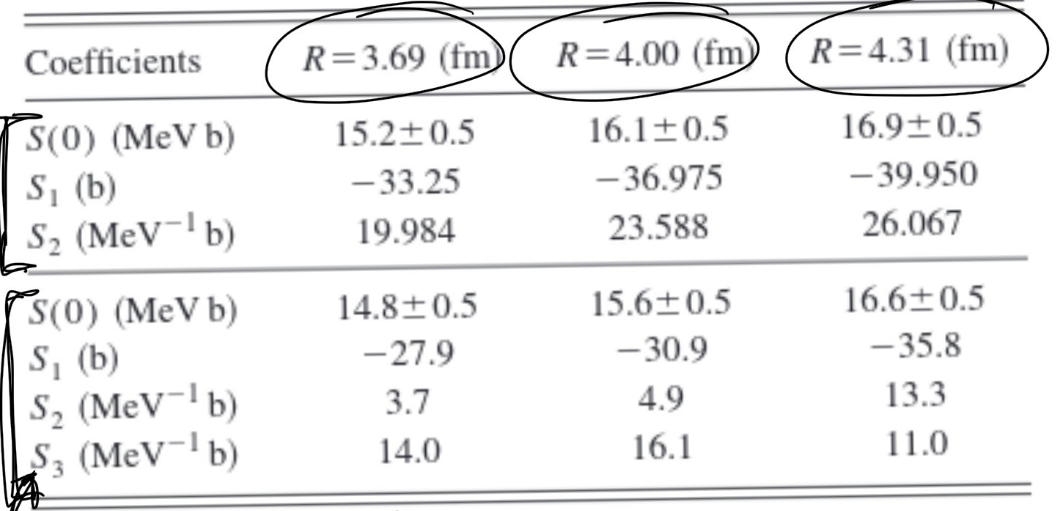
\includegraphics[scale=0.5]{Immagini/0421_tab.png}
	\caption{Valori dei parametri del fit per differenti raggi di \textit{cutoff}.}
	\label{0421_tab}
\end{figure}

\noindent Si ha così un fattore astrofisico compreso tra $14.8$ MeV$\,$b e $16.8$ MeV$\,$b e questo dimostrò che il metodo funzionava, dando una stima per $S(E)$ e il suo errore.
\newpage
\subsection{\textit{Asymptotic Normalization Coefficients method}}\index{Asymptotic Normalization Coefficients method@\textit{Asymptotic Normalization Coefficients method}}
\paragraph{Introduzione}
Consideriamo anche questa volta un nucleo fortemente a cluster\footnote{La notazione è stata cambiata} $B\equiv A+a$. L'equazione di \Sch{} ridotta per $A+a$ sarà:
$$u_L'' + \ppc{\frac{2\mu }{\hbar^2} V+ \frac{2\mu }{\hbar^2}E - \frac{L(L+1)}{r^2}}u_L =0$$
Prendiamo uno stato legato $E<0$ e definiamo $k\in \mathbb{C}$ tale $E\equiv \hbar^2 k^2 / 2\mu$, da cui $k = i\, \sqrt{2\mu |E|/\hbar^2} \equiv i\,k_I$ con $k_I\in \mathbb{R}$. Il potenziale sarà quello coulombiano più quello dovuto all'interazione nucleare $V=V_{nucl} + Z_1Z_2 e^2 /r$; definiamo allora il parametro:
$$\eta \equiv \frac{Z_1Z_2 e^2}{\hbar v} = \frac{Z_1Z_2 e^2}{\hbar}\frac{\mu}{\hbar k} = - i \, \frac{Z_1Z_2 e^2\mu}{\hbar^2 k_I} \equiv i\, \eta_I$$
%%! CAPIRE IL DISCORSO CHE SEGUE
A questo punto ci mettiamo a grande distanza ($V_{nucl} \simeq 0$ per $r>R_N$) e studiamo le soluzioni dell'equazione di \Sch{}, ovvero le funzioni di Coulomb\index{funzioni di Coulomb} \textit{in-going} e \textit{out-going}: $u^\pm_L (\eta,kr)$. In realtà, siccome siamo interessati solo alla soluzione asintotica prendiamo la \textit{in-going} perché vogliamo un andamento che sia $e^{ikr}=e^{-k_I r}$, dunque abbiamo solo $u^+_L(\eta,kr)$; questa però non è ben definita per $1+L+i\eta =0$, allora per correggere si usa la funzione di \Wh{}\index{funzione di \Wh}:
$$W_{-i\eta,L+1/2}(-2i\rho) = e^{-\pi\eta/2}e^{-i\,L\pi/2} u^+_L(\eta,\rho)$$
con $\rho\equiv kr$. Si può mostrare che per $r\to\infty$ ($\rho\to\infty$):
$$W_{-i\eta,L+1/2}(-2i\rho) \to e^{i\rho-i\eta\ln{2\rho}}\, e^{-\eta\pi/2} = \underbrace{e^{-k_Ir + \eta_I \ln{2k_Ir}}}_\text{Onda distorta}\: e^{i\eta_I\pi/2}$$
Dunque la nostra soluzione $u_L(r)$ asintoticamente sarà proporzionale a $W_{\eta_I,L+1/2}(2k_I r)$ e il fattore di proporzionalità $C_L$ viene appunto detto \textbf{Coefficiente Asintotico di Normalizzazione} (ANC)\index{Coefficiente Asintotico di Normalizzazione}.

\paragraph{Nel metodo}
Prendiamo la reazione:
$$b+c \to a+\gamma$$
in modo che sia perferica\index{reazione periferica}\footnote{Per quanto riguarda la notazione: con $\vec{\xi}_i$ indichiamo la posizione del nucleo $i$ rispetto all'origine (coordinate interne), con $\vec{r}$ invece indichiamo la distanza relativa tra il nucleo $b$ e il nucleo $c$.}, $E_{CM}\sim 0$: i nuclei $b$ e $c$ o si \vir{avvicinano poco} oppure entrano in interazione per breve tempo.\\ 
Sappiamo ormai che la sezione d'urto dipenderà dall'elemento di matrice:
\begin{align*}
	M 
	&= \oss{\psi_a}{\hat{\Theta}_\gamma}{\psi_{bc}^{scatt}} =\\
	&= \oss{\psi_a (\vec{\xi}_b,\vec{\xi}_c,\vec{r})}{\hat{\Theta}_\gamma (	\vec{r})}{\psi_{b}(\vec{\xi}_b)\psi_c(\vec{\xi}_c)\underbrace{\phi^+_{k_i}(\vec{r})}_\text{onda distorta}} =\\ 
	&= \oss{I_{bc}^a(\vec{r})}{\Theta_\gamma(\vec{r})}{\phi^+_{k_i}(\vec{r})}
\end{align*}
dove nell'ultimo passaggio abbiamo usato il fatto che l'operatore dipenda esclusivamente dalla distanza relativa $\vec{r}$ e quindi abbiamo integrato sulle coordinate interne, definendo:
$$
I_{bc}^a (\vec{r}) = \clebs{\psi_b(\vec{\xi}_b)\psi_c(\vec{\xi}_c)}{\psi_a(\vec{\xi}_b,\vec{\xi}_c,\vec{r})} = \sum_{\ell,m,S,S_z} i^\ell \, \clebs{J_bM_b,J_cM_c}{SS_z} \clebs{SS_z, \ell m}{J_aM_a} Y_{\ell m}(\hat{r})\:I_{bc,\ell s}^a (r)
$$
Questo ci permette di scrivere l'andamento asintotico della $\psi_a$ come una certa funzione di \textit{overlap}\footnote{Porta infatti l'informazione dell'\textit{overlap} tra la funzione d'onda di scattering $bc$ e quella di $a$.} $I_{bc,\ell s}^a (r)$; allora ci aspettiamo che asintoticamente ($r\gg R_N$) avremo (usando gli ANC per la ridotta):
$$I_{bc,\ell s}^a (r) \to \frac{C_{\ell s}}{r} \, W_{-i\eta,\ell+1/2} (2kr)$$%! che vuol dire -\eta ? 
Dunque se conosco gli ANC allora conosco anche $I$ e di conseguenza $M$.

\paragraph{Come trovare ANC} Esistono principalmente 2 modi:
\begin{itemize}
	\item calcolarli dalla teoria (non molto affidabili);
	\item oppure prenderli da altri esperimenti, dove si ha lo stesso vertice ($b+c \longleftrightarrow a$) e valgono le condizioni di reazione periferica.
\end{itemize}
\noindent Nel secondo caso si scelgono spesso reazioni di \textit{transfer} $b(X,Y)a$, con $X=Y+c$ cluster\footnote{Cambio di notazione.} (per cui il vertice è lo stesso).\\ 
Per fare un esempio prendiamo:
$$\underbrace{\ce{^{3}He}}_{p+d} + \ce{^{14}N} \to \ce{^{15}O}+\gamma + d$$
Sperimentalmente si misura $d\sigma^{transf}/d\Omega$ e questa è legata ai coefficienti di normalizzazione secondo:
$$\frac{d\sigma^{transf}}{d\Omega}\propto \sum_{J_x J_a} (C_{cY}^X)^2 (C_{bc}^a)^2 \sigma_\text{DWBA}$$
Se conosciamo $\sigma_\text{DWBA}$ e $C_{cY}^X$ otteniamo il valore cercato $C_{bc}^a$; $\sigma_\text{DWBA}$ si calcola facilmente, per quanto riguarda $C_{cY}^X$ si prende da un'altra reazione oppure si calcola (nel caso per esempio di $C_{pd}^{\ce{^3He}}$ è calcolabile).

\paragraph{Test case} Consideriamo la reazione:
$$p+\ce{^{16}O} \to \ce{^{17}F} + \gamma$$
per cui sono stati acquisiti dati diretti. Dobbiamo allora trovare il ANC di $\ce{^{17}F} \longleftrightarrow \ce{^{16}O} + p$ e a tale scopo prendiamo la reazione:
$$\ce{^{16}O} + \underbrace{\ce{^3He}}_{p+d} \to \ce{^{17}F} + d$$
con un fascio di $\ce{^3He}$ a $29.75$ MeV (reazione periferica). Si misura $d\sigma^{transf}/d\Omega$, si calcola\footnote{In realtà si tiene conto di un potenziale nucleare (spesso Wood-Saxon) a parametri liberi, così da poter valutare se la condizione di soluzione asintotica è ben soddisfatta: questa infatti, se asintotica, deve rimanere la stessa al variare dei parametri del potenziale.} $\sigma_\text{DWBA}$ e $C_{pd}^{\ce{^3He}}$.\\ 
I risultati sono riportati in Figura \ref{0421_OpgF} a sinistra per la distrubuzione angolare della reazione di \textit{transfer} e a destra per il fattore astrofisico da questa ottenuto; osserviamo che c'è sia uno stato fondamentale che un primo eccitato. Questo dimostra che il metodo funziona.

\begin{figure}[!h]
	\centering
	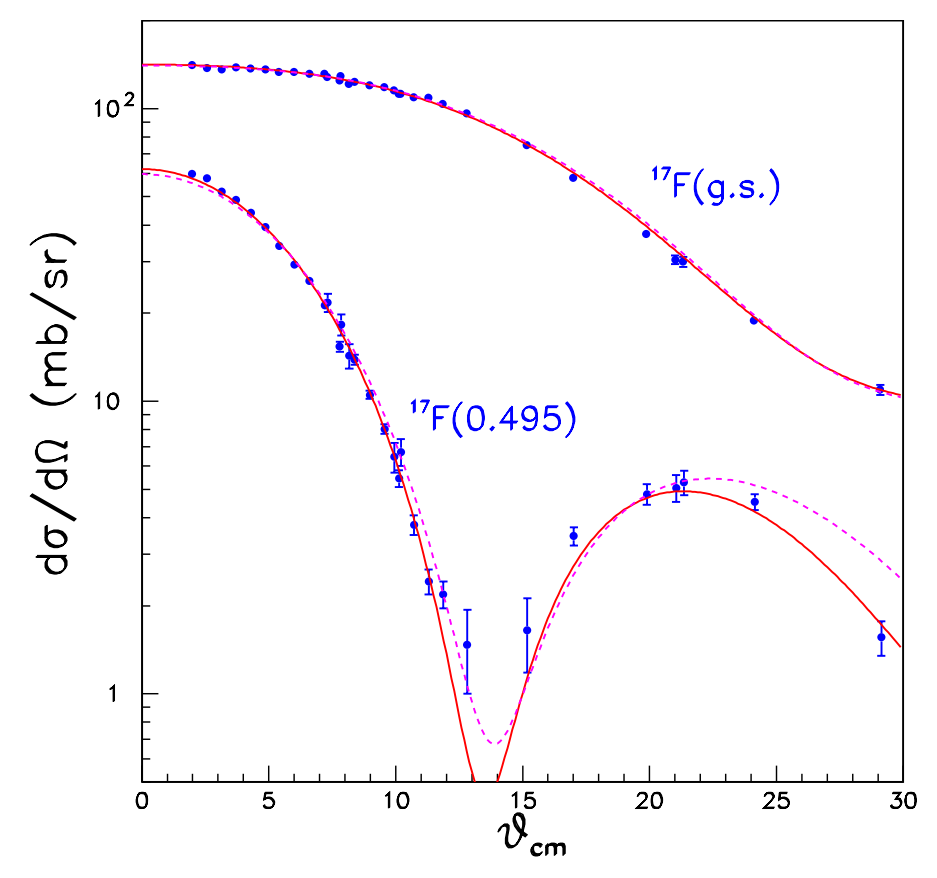
\includegraphics[scale=0.4]{Immagini/0421_theta.png}
	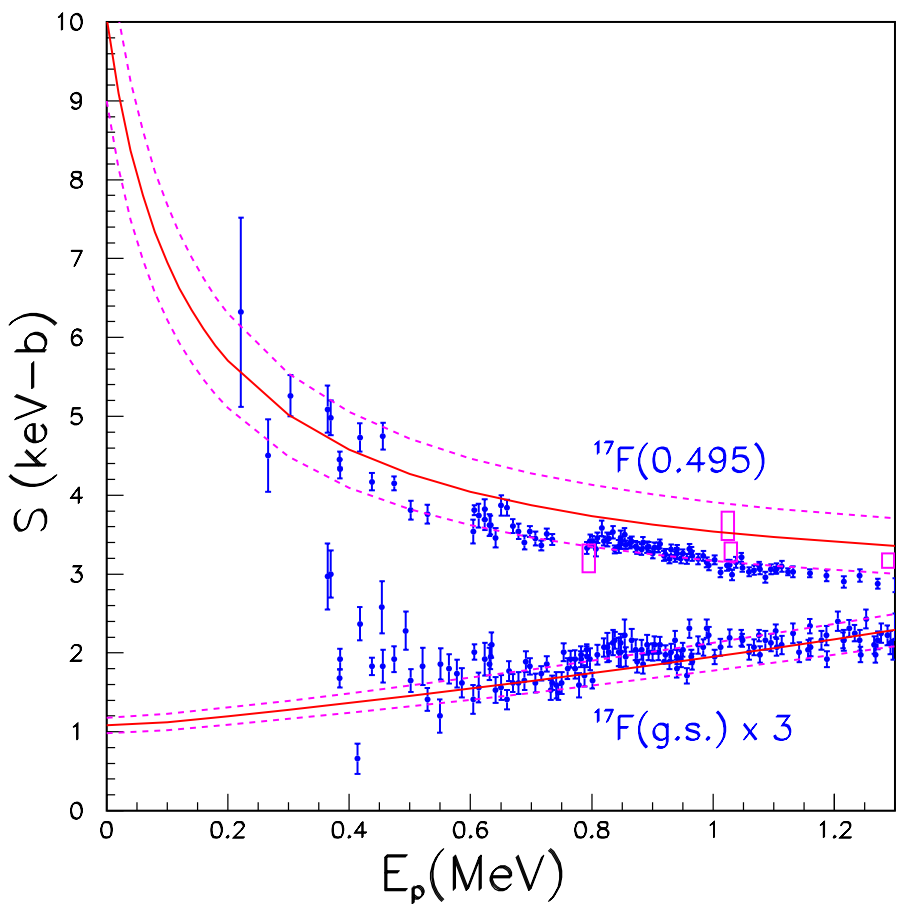
\includegraphics[scale=0.4]{Immagini/0421_Ep.png}
	\caption{A sinistra distribuzione angolare per la reazione $\ce{^{16}O}(\ce{^3He},d)\ce{^{17}F}$: le curve sono un fit in DWBA con parametri differenti; g.s. sta per \textit{ground-state}. A destra andamento del fattore astrofisico per $\ce{^{16}O}(p,\gamma)\ce{^{17}F}$: i puntini sono i dati delle misure dirette, mentre la curva rossa è ottenuta dagli ANC del grafico a sinistra.}
	\label{0421_OpgF}
\end{figure}

\paragraph{Il suo utilizzo} Il ANC \textit{method} fu usato per misurare la reazione:
$$p+\ce{^7Be}\to \ce{^8B}+\gamma$$
Ci sono varie opzioni per la reazione di \textit{transfer} da scegliere:
\begin{align*}
	-&\quad \ce{^7Be}(\ce{^3He},d)\ce{^8B} \\
	-&\quad \ce{^7Be}(\ce{^{10}B},\ce{^9Be})\ce{^8B} \\
	-&\quad \ce{^7Be}(\ce{^{14}N},\ce{^{13}C})\ce{^8B} 
\end{align*}
Per l'ultima è riportato il grafico della distribuzione angolare in Figura \ref{0421_BepgB} a sinistra. Si ottenne così un fattore astrofisico $S_{17}^{ANC}(0) = (18.0\pm 1.9)$ eVb compatibile con quello della misura diretta $S_{17}^{direct}(0) = (20.8\pm 0.7\pm 1.4)$ eVb, dati in Figura \ref{0421_BepgB} a destra. Notiamo che mentre per il CD \textit{method} in Figura \ref{0419_esp} non si osservava nessuna risonanza qui invece compare.


\begin{figure}[h]
	\centering
	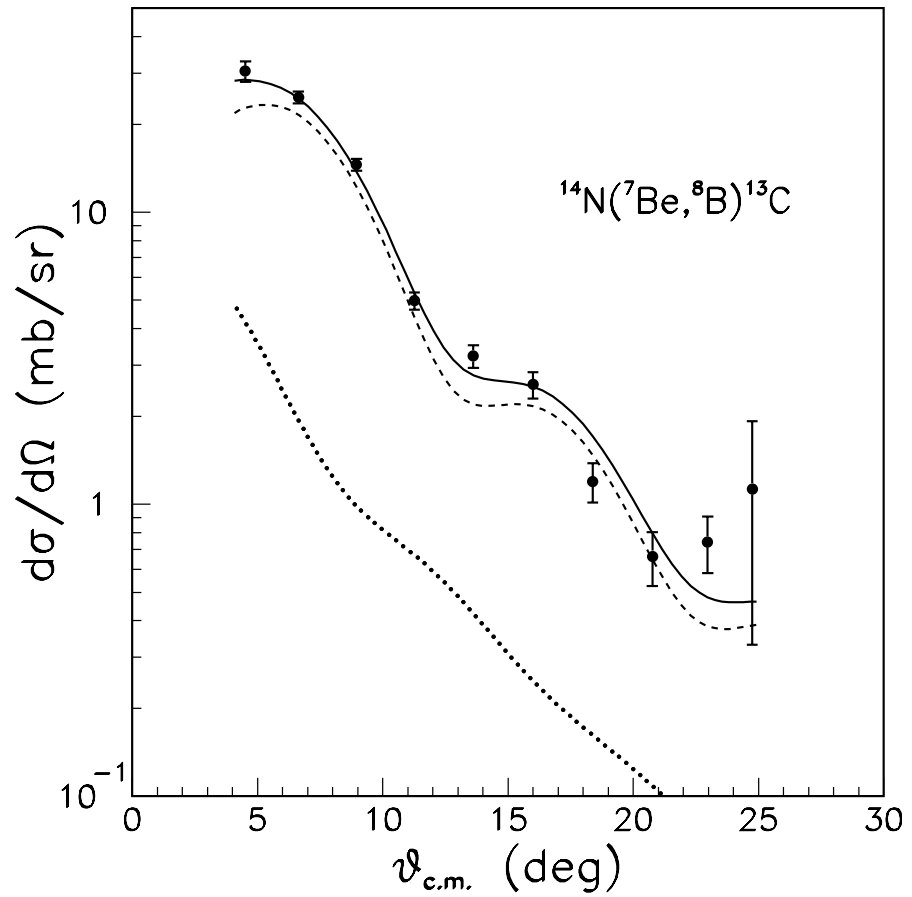
\includegraphics[scale=0.4]{Immagini/0421_theta2.png}
	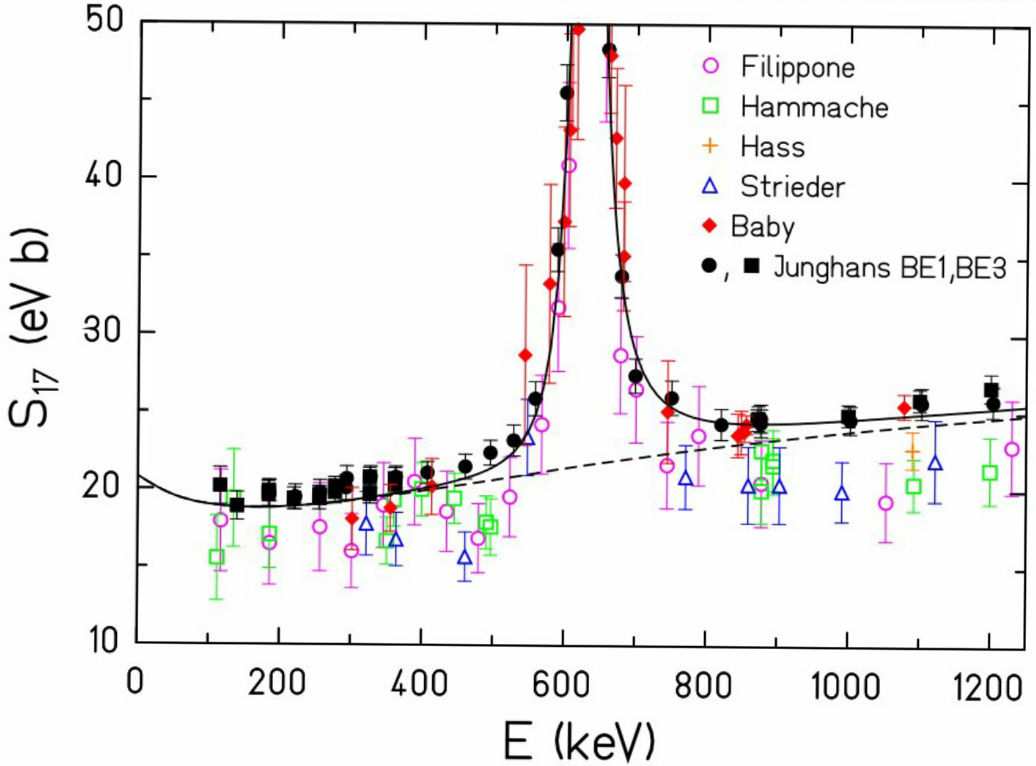
\includegraphics[scale=0.4]{Immagini/0421_E-keV.png}
	\caption{A sinistra distribuzione angolare della reazione $\ce{^{14}N}(\ce{^7Be},\ce{^8B})\ce{^{13}C}$: le linee rappresentano i fit in DWBA. A destra fattore astrofisico in funzione dell'energia ottenuto sia da misure dirette che con metodi indiretti.}
	\label{0421_BepgB}
\end{figure}



\chapter{Le ultime reazioni}
\section{La $3\alpha$}
Abbiamo studiato\footnote{Riguarda i capitoli \secrif{cap-BBN} e \secrif{cap-pp}.} che sia la catena $pp$\index{Catena protone-protone@Catena protone-protone $pp$} sia la BBN terminano con la produzione di particelle $\alpha$. Come avevamo già trattato nella sezione \secrif{sec-nuc-prim}, andare oltre sembra impossibile dal momento che non esistono nuclei legati per $A=5$ e quelli per $A=8$ decadono molto velocemente (\textit{mass gap}); tuttavia, le osservazioni mostrano che il $\ce{^{12}C}$ è il IV elemento più abbondante nell'universo.\\ 
La soluzione arrivò da Salpeter \& \"{O}pik: l'idea si basava sull'ipotesi che il carbonio si formasse in 2 \textit{step}.
\begin{enumerate}[1)]
	\item $\alpha +\alpha \to \ce{^8Be}$.\\ 
	Questo in realtà è instabile perché lo stato $0^+$ è sopra la soglia di $\alpha+\alpha$, $Q=92$ keV e $\tau_{dec}\sim \ord{-16}$ s. Se abbiamo $2\alpha$ con energia cinetica $T\sim Q$ allora $v= \sqrt{4Q/m_\alpha}\sim \ord{-2}\, c \simeq 3\cdot\ord{6}$ m/s; possiamo trovare un ordine di grandezza del tempo di transito prendendo la distanza di interazione $d\sim 3$ fm, per cui $t\sim d/v \sim \ord{-21}$ s$\lll \tau_{dec}$. Dunque, abbiamo una \vir{piccolissima} concetrazione di $\ce{^8Be}$ che sappiamo essere $N(\ce{^8Be})/N(\alpha)\simeq 5\cdot\ord{-10}$. Può avvenire allora il secondo \textit{step}.
	\item $\ce{^8Be + \alpha \to \ce{^{12}C} +\gamma}$.\\ 
	Si tratta di una cattura diretta, ma il fattore astrofisico sarebbe troppo piccolo per spiegare l'abbondanza di carbonio. Ecco che intervenne Hoyle: egli suppose che esistesse una risonanza per questo processo. A quel tempo quella di Hoyle fu una predizione perché non c'era modo di vederla; ormai è stata osservata e confermata: $J^{\pi}=0^+$ e $\Gamma_{tot} = (8.9\pm 1.08)$ eV (risonanza stretta), dove con $\Gamma_{tot}$ abbiamo indicato la larghezza del processo totale\footnote{Abbiamo considerato anche il processo di decadimento $\Gamma_\alpha$.} $\Gamma_{tot} = \Gamma_\alpha + \Gamma_{rad}\equiv \Gamma_\alpha + \Gamma_\gamma + \Gamma_{e^+e^-}$ .
	\begin{figure}[!h]
		\centering
		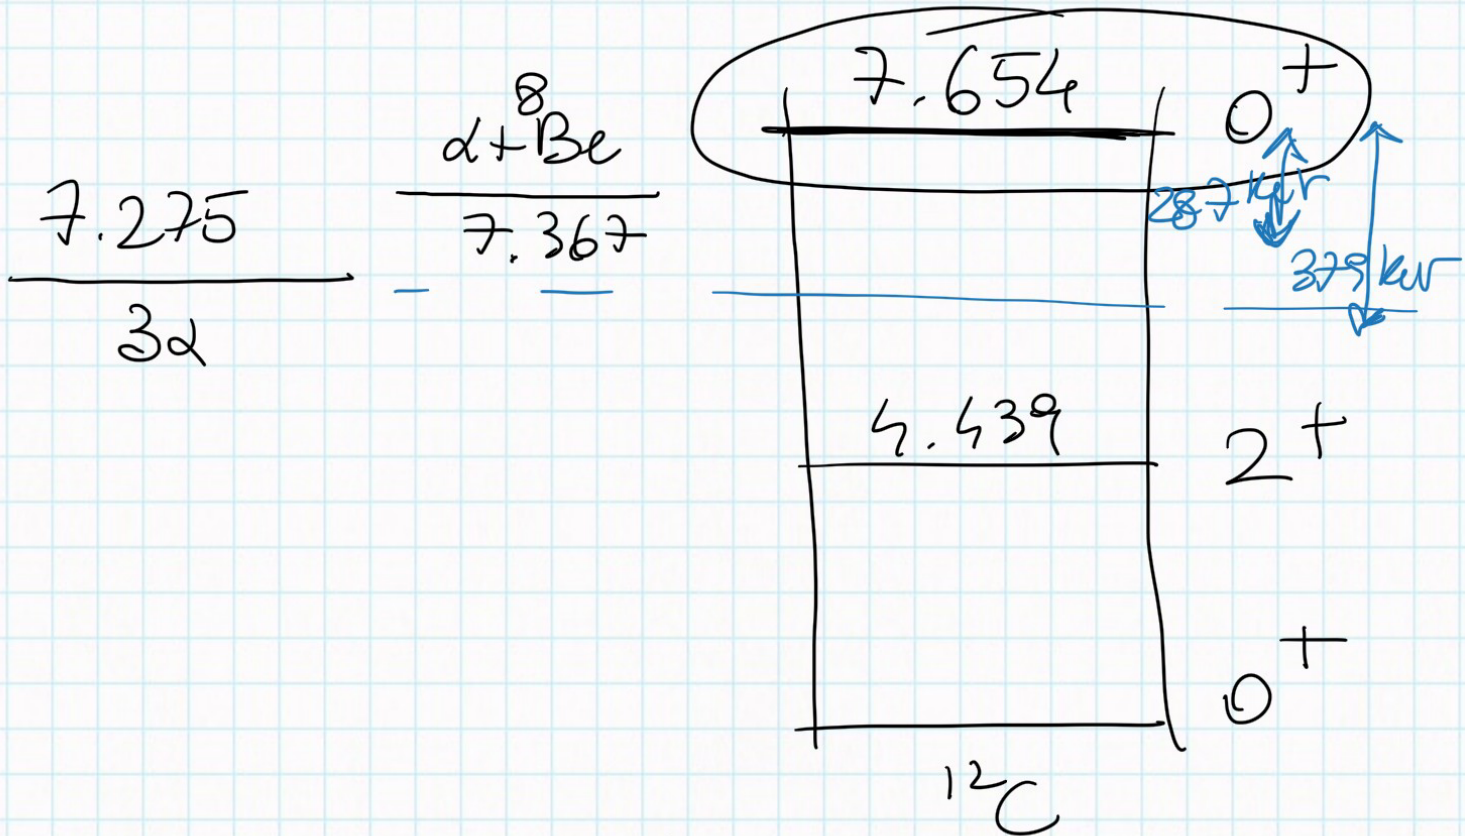
\includegraphics[scale=0.4]{Immagini/0421_riso.png}
		\caption{Livelli energetici per la risonanza di Hoyle della $3\alpha$.}
		\label{0421_hoyle}
	\end{figure}
\end{enumerate}
%%! CAPIRE MEGLIO QUANTO SEGUE
\noindent Per avere $0^+\to0^+$ non può esserci decadimento $\gamma$ perché per questo è vietata la transizione, mentre si può ottenere con produzione di coppia $e^+e^-$; tuttavia, è più probabile una transizione a 2 \textit{step}: $0^+\to2^+\to0^+$ ($E2+E2$). In questo caso $\Gamma_\gamma = (3.6\pm 0.5)$ meV$\ll \Gamma_\alpha$ ($E2$ è \vir{piccolo}). Dalla \BW{}:
$$\mean{\sigma v} = \ppc{\frac{2\pi}{\mu kT}}^{3/2} \hbar^2 \ppc{g \frac{\Gamma_\gamma\Gamma_\alpha}{\Gamma_{tot}}} e^{-E_R/kT}\simeq \ppc{\frac{2\pi}{\mu kT}}^{3/2} \hbar^2 \Gamma_\gamma\, e^{-E_R/kT}$$
dove abbiamo calcolato\footnote{$$g=\frac{2J+1}{2(2S_\alpha +1)} = 1 \qquad \text{per } 0^+$$} $g$ per $0^+$ e fatto l'approssimazione $\Gamma_{tot} \simeq \Gamma_\alpha$. Avremo allora per il rate:
$$r_{3\alpha} = N_{\ce{^8Be}}N_\alpha \, \mean{\sigma v}$$



